% ====================================================================================

\begin{frame}
\frametitle{1963 - Sketchpad by Ivan Sutherland}

\begin{columns}

    % Image on the left
    \begin{column}{0.48\textwidth}
        \centering
        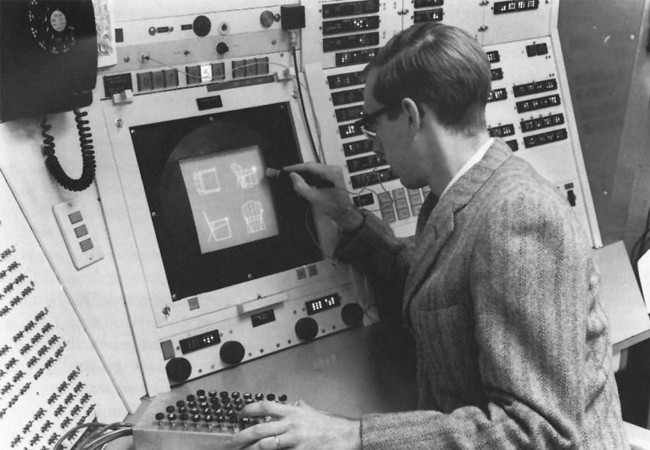
\includegraphics[width=\linewidth]{assets/sketchpad.jpg}
    \end{column}

    % Text on the right
    \begin{column}{0.48\textwidth}
        In 1963, Ivan Sutherland developed the Sketchpad for his doctoral thesis at MIT. This is important, since it was the first time that users could use a light-pen to draw shapes on a vector-based monitor. 
        Sutherland also introduced the concept of pop-up menus.
    \end{column}

\end{columns}

\end{frame}

% ====================================================================================

\begin{frame}
\frametitle{1963 - The Mouse by Doug Engelbart}

\begin{columns}

    % Image on the left
    \begin{column}{0.48\textwidth}
        \centering
        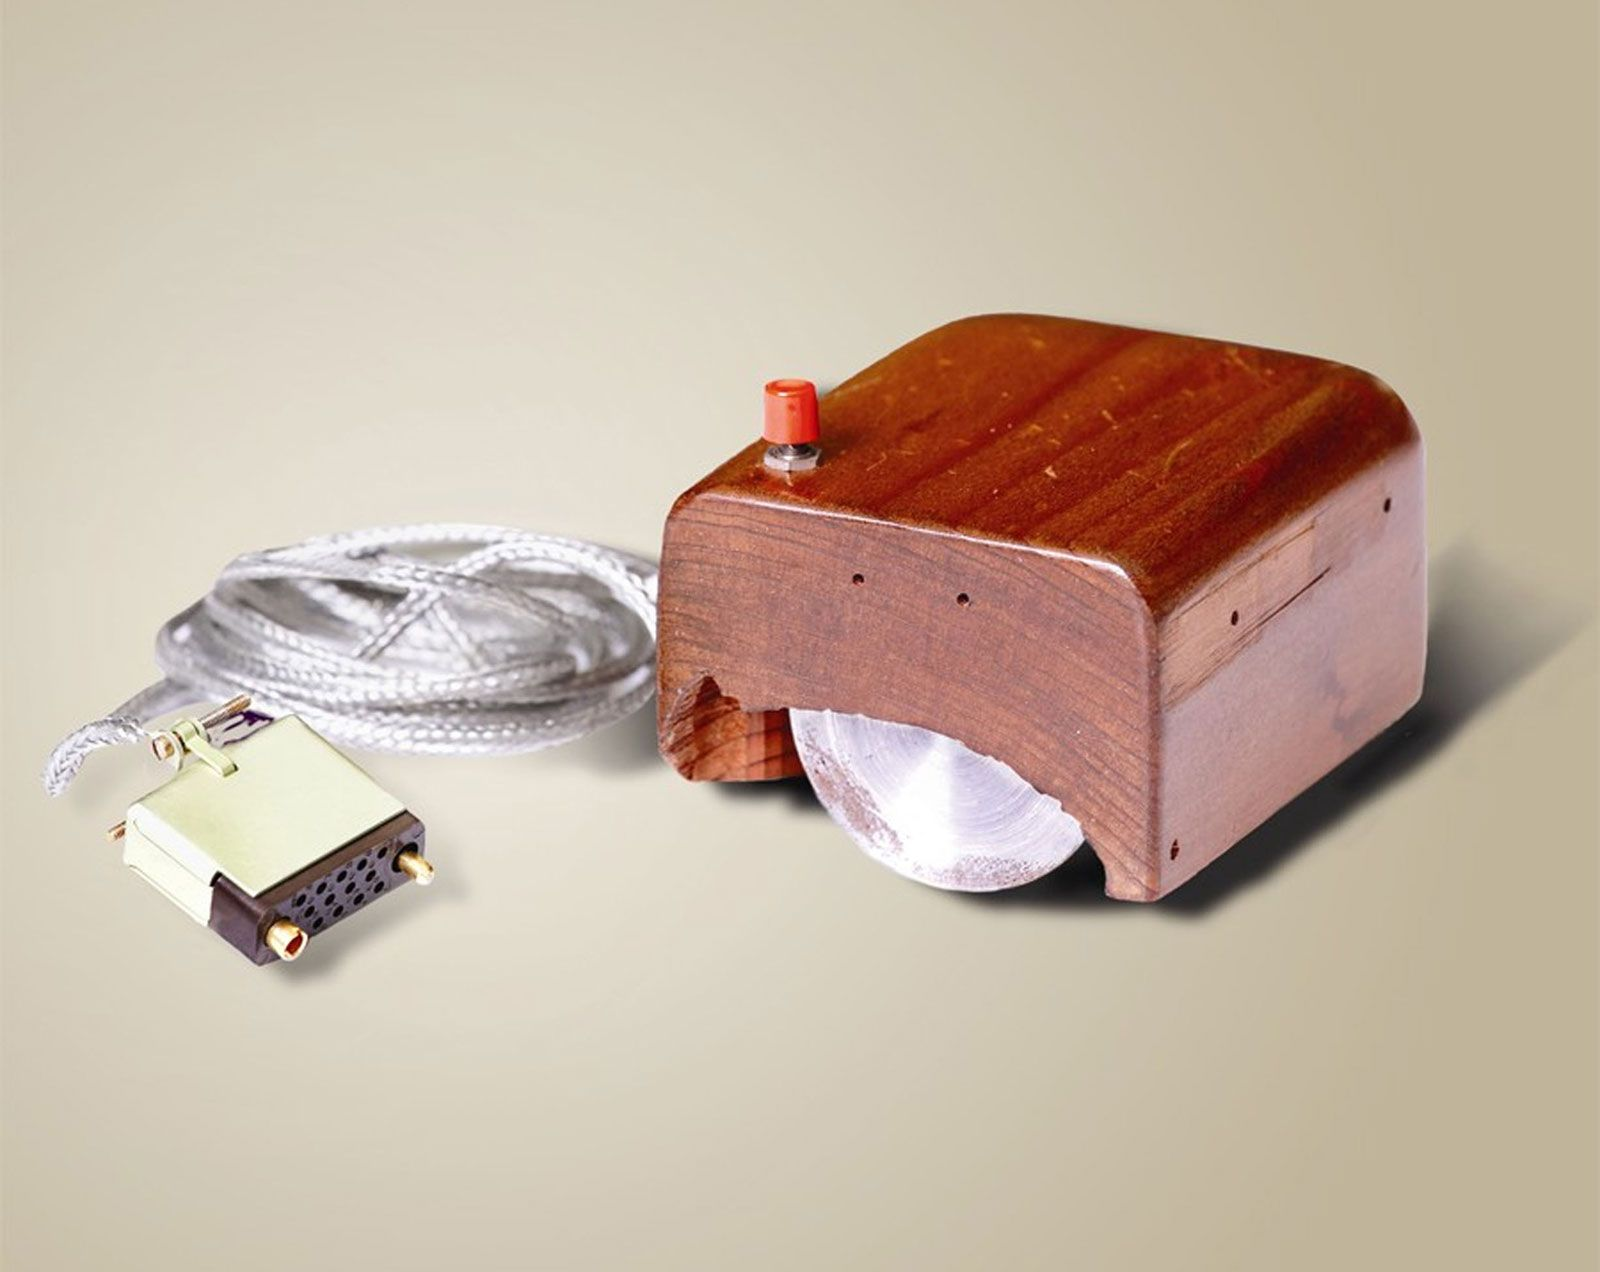
\includegraphics[width=\linewidth]{assets/mouse.jpg}
    \end{column}

    % Text on the right
    \begin{column}{0.48\textwidth}
        In 1963, Doug Engelbart invented the mouse at the Stanford Research Institute. The first prototype was made of a wooden shell, two wheels to track X-Y movements and a circuit-board.
    \end{column}

\end{columns}

\end{frame}

====================================================================================

\begin{frame}
\frametitle{1963 - The Hidden-Line Removal by Larry Roberts}

\begin{columns}

    % Image on the left
    \begin{column}{0.48\textwidth}
        \centering
        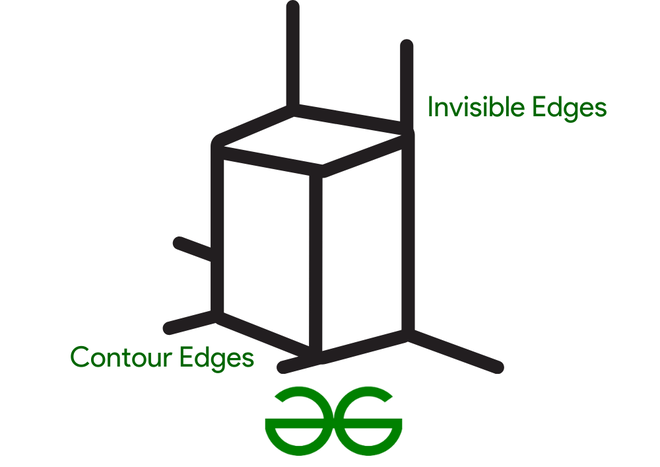
\includegraphics[width=\linewidth]{assets/hidden-line.png}
    \end{column}

    % Text on the right
    \begin{column}{0.48\textwidth}
        Contributing more to the 60s, Larry Roberts developed the first effective hidden-line removal algorithm. In simple words, it was an algorithm that removes the lines that should hidden in what it was supposed to be a 3D object. This algorithm helped to developed 3D objects rendering accurately.
    \end{column}

\end{columns}

\end{frame}